% https://www.tinkercad.com/things/5tth6OLRHPt-copy-of-kit-logico-modelo/editel?sharecode=SUnxTp9Fps-BiMfSit7VU2lw1o5RQNifgeI15UbR-yM
% https://www.tinkercad.com/things/hCCrtzcJJyE-roteiro3-parte-22/editel?sharecode=PtsZp45ElX69eXlrZ6RUbpy1vHVZd_---8yJ6dxY2TU
% https://www.tinkercad.com/things/69kCawlKX2i-roteiro3-parte-23/editel?sharecode=3Xug60JRRaJmdqFbfj94RdsFyIY3DcZ6AZmUIQGJKSs
% https://drive.google.com/drive/folders/1qmQaSxEHMEMgjFNUYUIII_uWlMOWUh7Z?usp=sharing

%%%%%%%%%%%%%%%%%%%%%%%%%%%%%%%%%%%%%%%%%%%%%%%%%%%%%%%%
% Este é um documento que servirá de modelo para
% os relatórios feitos na disciplina Laboratório de Circuitos Lógicos
% 2020-2
%%%%%%%%%%%%%%%%%%%%%%%%%%%%%%%%%%%%%%%%%%%%%%%%%%%%%%%%%

%%%%%%%%%%%%%%%%%%%%%%%%%%%%%%%%%%%%%%%%%%%%%%%%%%%%%%%%%
% Use os diferentes diretórios para colocar os relatórios de cada experimento, deste modo vc consegue manter um histórico e todo material organizado em apenas um local.
% Lembre-se de mudar o Main Document no Menu!!!

\documentclass[12pt]{article}

\usepackage{sbc-template}
\usepackage[brazil,american]{babel}
\usepackage[utf8]{inputenc}

\usepackage{graphicx}
\usepackage{url}
\usepackage{float}
\usepackage{listings}
\usepackage{color}
\usepackage{todonotes}
\usepackage{algorithmic}
\usepackage{algorithm}
\usepackage{hyperref}
\usepackage{amsmath}
\usepackage{graphicx}
\usepackage{array}
\usepackage[shortlabels]{enumitem}

\sloppy


\title{Experimento 4\\
Circuitos Combinacionais: Comparador de Palavras}

\author{Matheus Cardoso de Souza, 202033507\\
        Ualiton Ventura da Silva, 202033580\\
        Grupo G42
}

%%%% LEMBRE-SE DE MUDAR O GRUPO NA LINHA ABAIXO!!!!! %%%%%%
\address{Dep. Ciência da Computação -- Universidade de Brasília (UnB)\\
  CIC0231 - Laboratório de Circuitos Lógicos
  \email{matheus-cardoso.mc@aluno.unb.br, 202033580@aluno.unb.br}
}

\begin{document}
\maketitle

\selectlanguage{american}
 \begin{abstract}
   TODO
 \end{abstract}
\selectlanguage{brazil}

 \begin{resumo}
   TODO
 \end{resumo}


\section{Introdução}
\label{sec:Introducao}

% Escreva com suas palavras o que vai ser trabalhado no experimento. Aqui temos um exemplo de como citar a bibliografia consultada \cite{boulic:91} \cite{smith:99}.

TODO

\subsection{Objetivos}
\label{sec:Objetivos}

TODO

\subsection{Materiais}
\label{sec:Materiais}
Em função da natureza do ensino a distância, os presentes experimentos não foram
realizados usando-se materiais e equipamentos físicos, mas sim emulados por meio
do simulador online \href{https://www.tinkercad.com/}{Tinkercad}, e também do
\href{https://www.digitalelectronicsdeeds.com/deeds.html}{Deeds}.

A seguir estão enumerados os materiais simulados:
\begin{itemize}
    \item Painel Digital
    \item \textit{Protoboard}
    \item Fios
    \item Seletores de estado lógico
    \item LEDs
    \item Resistores
    \item Multímetros
    \item Portas Lógicas \textbf{NAND}
\end{itemize}

\section{Procedimentos}
\label{sec:Procedimentos}

Passaremos a apresentar os experimentos requeridos.

\subsection{Atraso de Propagação em portas lógicas}\label{sec:atraso_de_propagação}

\begin{enumerate}[A)]
\item \textbf{Equações Lógicas de \(L0\) e \(L1\)}
\end{enumerate}

Fazendo a tabela, temos:

\begin{table}[H]
    \centering
    \caption{Equações Lógicas de \(L0\) e \(L1\)}
    \begin{tabular}{|c|c|c|}\hline
        \multicolumn{1}{|c|}{Entrada} & \multicolumn{2}{|c|}{Saídas} \\\hline
        \textbf{A} & \textbf{\(L0\)} & \textbf{\(L1\)} \\\hline
        0 & 0 & 1 \\\hline
        1 & 0 & 0 \\\hline
    \end{tabular}\label{tab:atraso_de_propagação:L0_L1}
\end{table}

\begin{enumerate}[B)]
\item \textbf{Comportamento de \(L0\) e \(L1\)}
\end{enumerate}

Os LEDs \(L0\) e \(L1\) possuem o comportamento esperado.

\begin{figure}[H]
    \centering
    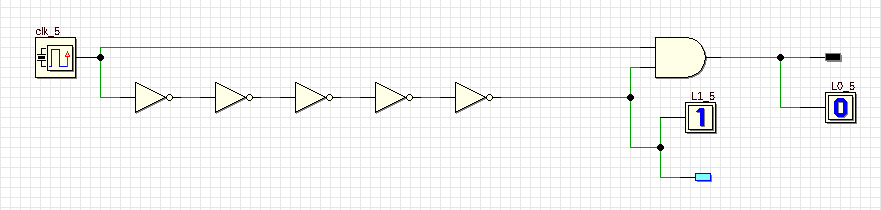
\includegraphics[width=.9\textwidth]{Exp04/exp4_2.0_b_clk_up.png}
    \caption{Clock Up}\label{fig:exp4_2.0_b_clk_up.png}
\end{figure}

\begin{figure}[H]
    \centering
    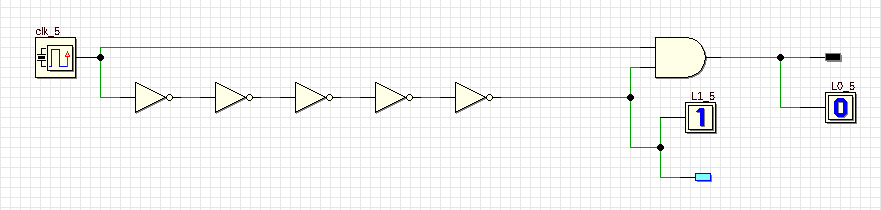
\includegraphics[width=.9\textwidth]{Exp04/exp4_2.0_b_clk_down.png}
    \caption{Clock Down}\label{fig:exp4_2.0_b_clk_down.png}
\end{figure}

\begin{enumerate}[C)]
\item \textbf{Formas de onda para \(L0\) e \(L1\)}
\end{enumerate}

\begin{figure}[H]
    \centering
    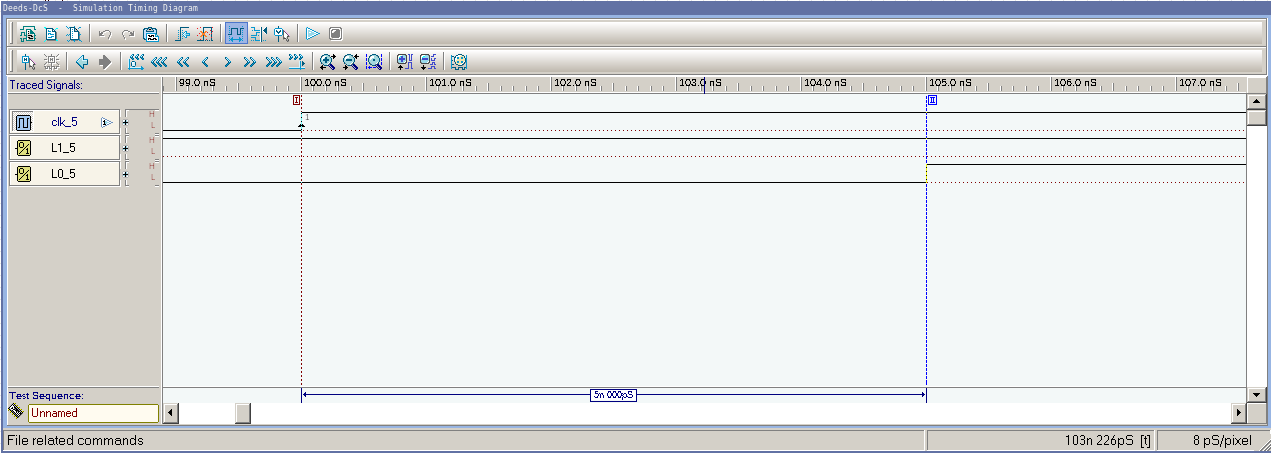
\includegraphics[width=.9\textwidth]{Exp04/exp4_2.0_c_clk_up.png}
    \caption{Clock Up}\label{fig:exp4_2.0_c_clk_up.png}
\end{figure}

\begin{figure}[H]
    \centering
    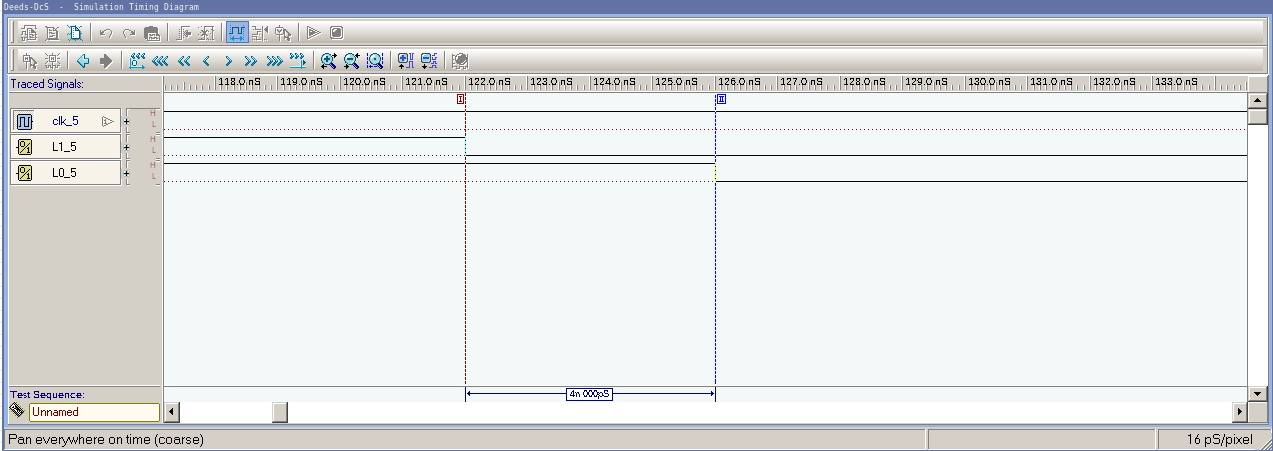
\includegraphics[width=.9\textwidth]{Exp04/exp4_2.0_c_clk_down.png}
    \caption{Clock Down}\label{fig:exp4_2.0_c_clk_down.png}
\end{figure}

\begin{enumerate}[D)]
\item \textbf{Motivo de pulsos em \(L0\)}
\end{enumerate}

Delay

\begin{enumerate}[E)]
\item \textbf{Haveria pulso em \(L0\) caso houvesse um número par de portas \textbf{NOT}?}
\end{enumerate}

Sim, só depende se a quantidade de portas \textbf{NOT} é suficiente para
introduzir um delay suficientemente grante.

\subsection{Comparador de palavras de \(3\) \emph{bits}}\label{sec:comparador_de_palavras_3_bits}

Completando a tabela para o circuito \textbf{XNOR}, temos:

\begin{table}[H]
    \centering
    \caption{Tabela Verdade para o circuito \textbf{XNOR}}
    \begin{tabular}{|c|c|c|c|c|}\hline
    \multicolumn{2}{|c|}{Entradas} & \multicolumn{1}{|c|}{Saída} \\\hline
    \textbf{$A_{i}$} & \textbf{$B_{i}$} & \textbf{$Z_{i}$} \\\hline
    0 & 0 & 1 \\\hline
    0 & 1 & 0 \\\hline
    1 & 0 & 0 \\\hline
    1 & 1 & 1 \\\hline
    \end{tabular}\label{tab:comparador_de_palavras_3_bits}
\end{table}


\section{Análise dos Resultados}
\label{sec:Resultados}

TODO

\section{Conclusão}
\label{sec:Conclusao}

TODO

\nocite{*}
\bibliographystyle{sbc}
\bibliography{relatorio}  %Aqui é a definição do arquivo .bib a ser usado pelas referências


\newpage
% Colocar aqui apenas as respostas dos itens da Auto-Avaliação
\section*{Auto-Avaliação}

Respostas:

TODO
% \begin{table}[H]
%     \begin{tabular}{|c|c|} \hline
%     \textbf{A} & \textbf{B}\\
%     \hline
%     1 & b \\ \hline
%     2 & d \\ \hline
%     3 & c \\ \hline
%     4 & a \\ \hline
%     5 & d \\ \hline
%     \end{tabular}
% \end{table}


\end{document}
